\documentclass[12pt]{article}
\usepackage{fullpage}
\usepackage{enumitem}
\usepackage{amsmath}
\usepackage{amssymb}
\usepackage{graphicx}
\usepackage{bm}
\usepackage{hyperref}

\begin{document}

\begin{center}
{\Large CS224n Winter 2019 Homework 2: word2vec}

\begin{tabular}{rl}
SUNet ID: & 05794739 \\
Name: & Luis Perez \\
Collaborators: &
\end{tabular}
\end{center}

By turning in this assignment, I agree by the Stanford honor code and declare
that all of this is my own work.

\section*{Problem 1}
\begin{enumerate}[label=(\alph*)]
\item The key insight for this equality is that the vector of the true distribution $\bm{y}$ is one-hot encoded vector with $1$ for the true, outside word $o$ and $0$ everywhere else. We therefore have:
\begin{align*}
\text{CrossEntropy}(\bm{y}, \bm{\hat{y}}) &= - \sum_{w \in Vocab} y_w \log(\hat{y}_w) \\
&= -1 \cdot \log(\hat{y}_o) - \sum_{w \in Vocab, w \neq o} 0 \cdot \log(\hat{y}_w)\\
&= -\log(\hat{y}_o) \\
&= -\log P(O = o \mid C = c) = \bm{J}_{\text{naive-softmax}}(\bm{v}_c, o, \bm{U})
\end{align*}

\item We compute the partial derivate of the cross-entropy loss with respect to $v_c$.
\begin{align*}
\frac{\partial J}{\partial \bm{v}_c} &= -\frac{\partial}{\partial \bm{v}_c} \left[ \sum_{w \in Vocab} \bm{y}_w \log \bm{\hat{y}}_w \right] \tag{Results from 1a} \\
&= -\sum_{w \in Vocab} \bm{y}_w \frac{\partial}{\partial \bm{v}_c} \log \frac{\exp{\bm{u}_w^T\bm{v}_c}}{\sum_{k \in Vocab} \exp{\bm{u}_k^T \bm{v}_c}} \tag{Definition of $\bm{\hat{y}}_w$} \\
&= -\sum_{w \in Vocab} \frac{\bm{y}_w}{\bm{\hat{y}}_w} \frac{\partial}{\partial \bm{v}_c} \frac{\exp{\bm{u}_w^T} \bm{v}_c}{\sum_{k \in Vocab} \exp{\bm{u}_k^T \bm{v}_c}} \tag{Derivative of $\log x$ and Chain rule} \\
&= - \sum_{w \in Vocab} \frac{\bm{y}_w}{\bm{\hat{y}}_w} \left[ \frac{\bm{u}_w\exp(\bm{u}_w^T \bm{v}_c)\sum_{k \in Vocab} \exp \bm{u}_k^T \bm{v}_c}{\left(\sum_{k \in Vocab} \exp \bm{u}_k^T \bm{v}_c \right)^2} - \frac{\exp(\bm{u}_w^T \bm{v}_c)\sum_{k \in Vocab} \bm{u}_k \exp \bm{u}_k^T \bm{v}_c}{\left(\sum_{k \in Vocab}\exp \bm{u}_k^T\bm{v}_c \right)^2} \right] \tag{Quotient Rule of Derivates} \\
&= -\sum_{w \in Vocab} \frac{\bm{y}_w}{\bm{\hat{y}_w}} \left[\bm{u}_w \bm{\hat{y}}_w - \bm{\hat{y}}_w \sum_{k \in Vocab} \frac{\bm{u}_k \exp{\bm{u}_k^T \bm{v}_c}}{\sum_{\ell \in Vocab} \exp{\bm{u}_{\ell}^T \bm{v}_c}} \right] \tag{Simplification using definition of $\hat{\bm{y}}_w$, reindex sum} \\
&= -\sum_{w \in Vocab} \bm{y}_w \bm{u_w} + \left(\sum_{w \in Vocab} \bm{y}_w\right)\left(\sum_{k \in Vocab} \bm{u}_k \bm{\hat{y}}_k  \right) \tag{Defintion of $\bm{\hat{y}}_k$, distribute sum, simplify} \\
&= \bm{U}[\hat{\bm{y}} - \bm{y}] \tag{Convert to matrix form.}
\end{align*}

\item We compute the partial derivate of the cross-entry loss with respect to $\bm{u}_w$. We have:
\begin{align*}
 \frac{\partial J}{\partial \bm{u}_w} &= -\frac{\partial}{\partial \bm{u}_w} \left[ \sum_{k \in Vocab} \bm{y}_k \log \bm{\hat{y}}_k \right] \tag{Results from 1a} \\
&= -\sum_{k \in Vocab} \bm{y}_k \frac{\partial}{\partial \bm{u}_w} \log \frac{\exp{\bm{u}_w^T\bm{v}_c}}{\sum_{k \in Vocab} \exp{\bm{u}_k^T \bm{v}_c}} \tag{Definition of $\bm{\hat{y}}_k$} \\
&= -\sum_{k \in Vocab} \frac{\bm{y}_k}{\bm{\hat{y}}_k} \frac{\partial}{\partial \bm{u}_w} \frac{\exp{\bm{u}_k^T} \bm{v}_c}{\sum_{\ell \in Vocab} \exp{\bm{u}_{\ell}^T \bm{v}_c}} \tag{Derivative of $\log x$ and Chain rule} \\
&= -\frac{\bm{y}_w}{\bm{\hat{y}}_w} \frac{\bm{v}_c \exp(\bm{u}_w^T \bm{v}_c) \sum_{\ell \in Vocab} \exp \bm{u}_{\ell}^T \bm{v}_c - \bm{v}_c \left(\exp{\bm{u}_w^T \bm{v}_c}\right)^2 }{\left(\sum_{\ell \in Vocab} \exp \bm{u}_{\ell}^T \bm{v}_c \right)^2} \\
&+ \sum_{k \in Vocab, k \neq w} \frac{\bm{y}_k}{\bm{\hat{y}}_k}\frac{\bm{v}_c \exp{(\bm{u}_w^T \bm{v}_c)}\exp{(\bm{u}_k^T \bm{v}_c)}}{\left(\sum_{\ell \in Vocab} \exp{\bm{u}_{\ell}^T} \bm{v}_c \right)^2} \tag{Quotient Rule and split into cases} \\
&= -\bm{v}_c\bm{y}_w \left[1 - \bm{\hat{y}}_w \right] + \bm{v}_c \sum_{k \in Vocab, k \neq w} \bm{y}_k \bm{\hat{y}}_w \tag{Simplify} \\
&= [-\bm{y}_w + \bm{\hat{y}}_w(\bm{y}_w + \sum_{k \in Vocab, k \neq w} \bm{y}_k) ] \bm{v}_c \tag{Refactoring} \\
&= [\bm{\hat{y}}_w - \bm{y}_w]\bm{v}_c
\end{align*}
We can, in fact, write the above for the entire matrix $\bm{U}$ as follows:
$$
\frac{\partial J}{\partial \bm{U}} = \bm{v}_c[\bm{\hat{y}} - \bm{y}]^T
$$

\item We compute the derivative element by element. We have: 
\begin{align*}
\frac{d}{d\bm{x}_i} \sigma(\bm{x}_i) &= \frac{d}{d\bm{x}_i} \left[ \frac{e^{\bm{x}_i}}{1 + e^{\bm{x}_i}} \right] \\
&= \frac{e^{\bm{x}_i}(1 + e^{\bm{x}_i}) - e^{\bm{x}_i}\cdot e^{\bm{x}_i}}{(1 + e^{\bm{x}_i})^2} \\
&= \left(\frac{e^{\bm{x}_i}}{1 + e^{\bm{x}_i}}\right)\left(1 - \frac{e^{\bm{x}_i}}{1 + e^{\bm{x}_i}} \right) \\
&= \sigma(x_i)[1 - \sigma(x_i)]
\end{align*}
As such, we have the vector derivate as:
$$
\frac{d}{d \bm{x}} \sigma(\bm{x}) = \sigma(\bm{x}) \circ [\bm{1} - \sigma(\bm{x})]
$$
where $\circ$ represents element-wise vector product.

\item We compute the requested derivatives for the negative sampling loss function. First, with respect to $\bm{u}_o$.
\begin{align*}
\frac{\partial J}{\partial \bm{u}_o} &= - \frac{\partial}{\partial \bm{u}_o} \log \sigma(\bm{u}_o^T \bm{v}_c)  \tag{Only the first term depends on $\bm{u}_o$} \\
&= -\frac{\sigma(\bm{u}_o^T \bm{v}_c)(1 - \sigma(\bm{u}_o^T \bm{v}_c))}{\sigma(\bm{u}_o^T\bm{v}_c)} \bm{v}_c \tag{Derivative of $\log x$ and results from 1d} \\
&= -(1 - \sigma(\bm{u}_o^T \bm{v}_c)) \bm{v}_c
\end{align*}
Next, with respect to $\bm{u}_k$.
\begin{align*}
\frac{\partial J}{\partial \bm{u}_k} &= - \frac{\partial}{\partial \bm{u}_k} \log \sigma(-\bm{u}_k^T \bm{v}_c)  \tag{Only the $k+1$-th term depends on $\bm{u}_k$} \\
&= \frac{\sigma(-\bm{u}_k^T \bm{v}_c)(1 - \sigma(-\bm{u}_k^T \bm{v}_c))}{\sigma(-\bm{u}_k^T\bm{v}_c)} \bm{v}_c \tag{Derivative of $\log x$ and results from 1d} \\
&= (1 - \sigma(-\bm{u}_k^T \bm{v}_c)) \bm{v}_c
\end{align*}
And finally, with respect to $\bm{v}_c$.
\begin{align*}
\frac{\partial J}{\partial \bm{v}_c} &= - \frac{\partial}{\partial \bm{v}_c} \log \sigma(\bm{u}_o^T \bm{v}_c) - \sum_{k=1}^K \frac{\partial}{\partial \bm{v}_c} \log \sigma(-\bm{u}_k^T \bm{v}_c)  \\
&= -(1 - \sigma(\bm{u}_o^T \bm{v}_c))\bm{u}_o + \sum_{k=1}^K (1 - \sigma(-\bm{u}_k^T \bm{v}_c)) \bm{u}_k \tag{Previous results} 
\end{align*}
Computing the naive-softmax requires iterating over the entire vocabulary, which can be extremely large, while the negative sampling loss requires considering only $K+1$ samples.

\item We now compute the skip-gram loss function. We have:
\begin{enumerate}[label=\roman*]
  \item 
  $$
  \frac{\partial \bm{J}_{\text{skip-gram}}(\bm{v}_c, w_{t-m}, \cdots, w_{t+m}, \bm{U})}{\partial \bm{U} } = \sum_{\substack{-m \leq j \leq m \\ j \neq 0}} \frac{\partial \bm{J}(\bm{v}_c, w_{t+m}, \bm{U}) }{\partial \bm{U}}
  $$
  \item 
  $$
  \frac{\partial \bm{J}_{\text{skip-gram}}(\bm{v}_c, w_{t-m}, \cdots, w_{t+m}, \bm{v}_c)}{\partial \bm{v}_c } = \sum_{\substack{-m \leq j \leq m \\ j \neq 0}} \frac{\partial \bm{J}(\bm{v}_c, w_{t+m}, \bm{U}) }{\partial \bm{v}_c}
  $$
  \item
  \begin{align*}
  \frac{\partial \bm{J}_{\text{skip-gram}}(\bm{v}_c, w_{t-m}, \cdots, w_{t+m}, \bm{v}_c)}{\partial \bm{v}_w }  = 0 \tag{$w \neq c$}
  \end{align*}
\end{enumerate}
\end{enumerate}

\section*{Problem 2}
\begin{enumerate}[label=(\alph*)]
  \item In `word2vec.py'
  \item In `sgd.py'
  \item Using `run.py' we get Figure \ref{fig:projection}. The plot shows the projection of our learned word vectors into two dimensions.

  We see a few clusters forming -- such as adjectives (``amazing'', ``wonderful'', ``great'', ``boring'') -- which, not surprisingly, contain not only synonyms but also antonyms. We also see a few other interesting clusters, such as ``queen'' and ``dumb'' (surprising, and sexist) as well as ``female'' and ``woman'' (not surprising). Lastly, we see ``hail'' as a single, unclustered word, which is a bit surprising given what we would intuitively expect (to cluster with ``snow'', ``rain'' as a weather phenomena).
    \begin{figure}[!h]
      \centering
      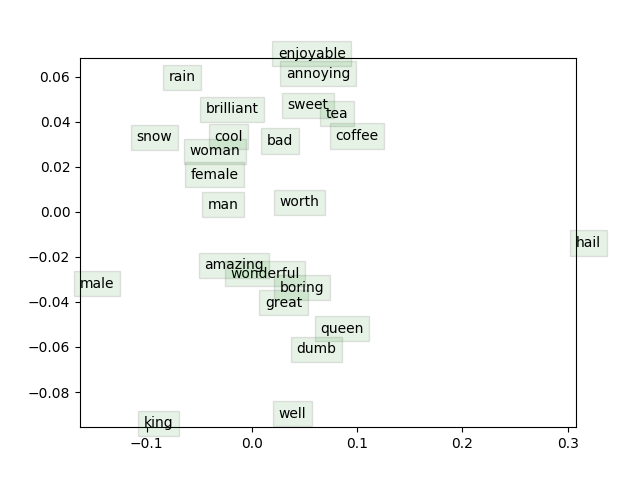
\includegraphics[]{../word_vectors.png}
      \caption{Projection of word2vec embeddings.}
      \label{fig:projection}
    \end{figure}
\end{enumerate}

































\end{document}